\documentclass[12pt,letterpaper,final]{article}

\usepackage{Sweave}
\usepackage{graphicx}
\usepackage{natbib}
\usepackage{hyperref}
\usepackage{caption}
\usepackage{rotating}
\usepackage{verbatim}
\usepackage{textcomp}
\usepackage{wasysym}

\setlength{\oddsidemargin}{0in}
\setlength{\textwidth}{6.15in}
%\setlength{\topmargin}{0.5in}
\setlength{\textheight}{22cm}
\setlength{\headheight}{0in}
\setlength{\headsep}{0in}
\setlength{\parskip}{5pt plus 2pt minus 3pt}

\def\thefootnote{\fnsymbol{footnote}}
\setcounter{footnote}{1}

\renewcommand{\baselinestretch}{1.2}
\renewcommand{\labelenumi}{(\roman{enumi})}

\renewcommand{\topfraction}{1.0}
\renewcommand{\bottomfraction}{1.0}
\renewcommand{\textfraction}{0.0}
\renewcommand{\floatpagefraction}{1.0}

\newtheorem{definition}{Definition}
\newtheorem{theorem}{Theorem}
\newtheorem{lemma}[theorem]{Lemma}
\newtheorem{claim}[theorem]{Claim}
\newtheorem{fact}[theorem]{Fact}

% to get nice proofs ...
\newcommand{\qedsymb}{\mbox{ }~\hfill~{\rule{2mm}{2mm}}}
\newenvironment{proof}{\begin{trivlist}
\item[\hspace{\labelsep}{\bf\noindent Proof: }]
}{\qedsymb\end{trivlist}}


\newfont{\msymb}{cmsy10 scaled 1000}

\def\nullset{\mbox{\O}}
\def\R{{I\!\!R}}
\def\C{{I\!\!\!\!C}}
\def\N{{I\!\!N}}

\def\P{\mbox{\msymb P}}


%\parskip 0.1in
\pagenumbering{arabic}    %  Start using 1,2,... as page numbers.
\pagestyle{plain}         %  Page numbers in middle bottom of page.
%\setcounter{page}{80}  % XXXXXXXXXXXXXXXXX
%\setcounter{theorem}{5} % XXXXXXXXXXXXXXXXX
%\setcounter{definition}{10} % XXXXXXXXXXXXXXXXX

\parindent 0in


\begin{document}

\Sconcordance{concordance:hw02_bartschi.tex:hw02_bartschi.Rnw:%
1 116 1 1 2 1 0 8 1 3 0 1 2 8 1 1 2 5 0 1 2 11 1 1 2 1 0 1 1 1 5 3 0 1 %
5 3 0 1 5 3 0 1 5 3 0 1 2 4 0 1 2 12 1 1 8 11 0 1 2 9 1 1 2 1 0 1 1 1 2 %
1 0 1 2 1 0 1 2 1 0 1 2 5 0 1 2 17 1 1 13 12 0 1 12 11 0 1 12 11 0 1 12 %
11 0 1 12 11 0 1 12 11 0 1 2 4 0 1 2 17 1 1 6 5 0 1 7 6 0 1 6 5 0 1 1 4 %
0 1 2 13 1 1 5 8 0 1 2 8 1 1 5 8 0 1 2 44 1 1 2 1 0 1 1 4 0 2 2 5 0 2 2 %
5 0 2 2 5 0 2 2 5 0 2 2 5 0 1 2 13 1 1 2 5 0 1 2 26 1 1 2 1 0 1 3 6 0 1 %
2 52 1}


\begin{titlepage}
\vspace*{4.5cm}
\begin{center}
{\LARGE \bf Stat 5810, Section 003} \\[0.5cm]
{\LARGE \bf Statistical Visualization I} \\[0.5cm]
{\LARGE \bf Fall 2018} \\[0.5cm]
{\LARGE \bf Homework 2} \\[0.5cm]
~ \\[2cm]
{\bf ShaunMicheal Bartschi} \\[0.3cm]
{A01975136} \\[0.3cm]
{November 27, 2018} \\[0.3cm]
\end{center}

\thispagestyle{empty}
\vfill
\end{titlepage}

\begin{table}\centering
\begin{tabular*}{6.15in}{@{\extracolsep{\fill}}|llr|} \hline
Stat 5810 Statistical Visualization I & \hspace*{0.5 in} & Fall 2018 \\
 & & \\
\multicolumn{3}{|c|}{
Homework Assignment 2 (11/3/2018)} \\
 & & \\
\multicolumn{3}{|c|}{
65 Points --- Due Tuesday 11/27/2018 (via Canvas by 11:59pm)} \\
\hline
\end{tabular*}
\end{table}


\begin{enumerate}


\item (39 Points) {\bf Olive Oils from Italy:}
In this question, you have to work with the {\it olives} data set from the {\it extracat} package.
We are only interested in the variables {\it palmitic} and {\it Region}
in this question. Ignore all other variables.
See the {\it olives} help page for further details.


\begin{enumerate}
\item (2 Points) 
Load all required R packages to answer this question. Show your R code.
Do not just blindly trust the information on the help page! How many observations are included 
in this data set overall? And how many are there in each of the three regions?\\

\underline{Answer:}
{\scriptsize
\begin{Schunk}
\begin{Sinput}
> setwd("C:/Users/Shaun/Desktop/StatVis/HW2")
> library(ggplot2)
> library(ggthemes)
> library(grid)
> library(gridExtra)
> library(extracat)
> library(lvplot)
> library(lattice)
> data(olives)
\end{Sinput}
\end{Schunk}
It appears that there are 572 observations in the data set, with 151 observations in the North, 98 observations in Sardinia, 323 observations in the South.
}


\item (3 Points) 
Create a default histogram via {\it ggplot2}. Do not optimize
this histogram. Describe this histogram. 
Include your figure and your R code. \\

\begin{Schunk}
\begin{Sinput}
> ggplot(olives,aes(x = palmitic)) + geom_histogram()
\end{Sinput}
\end{Schunk}
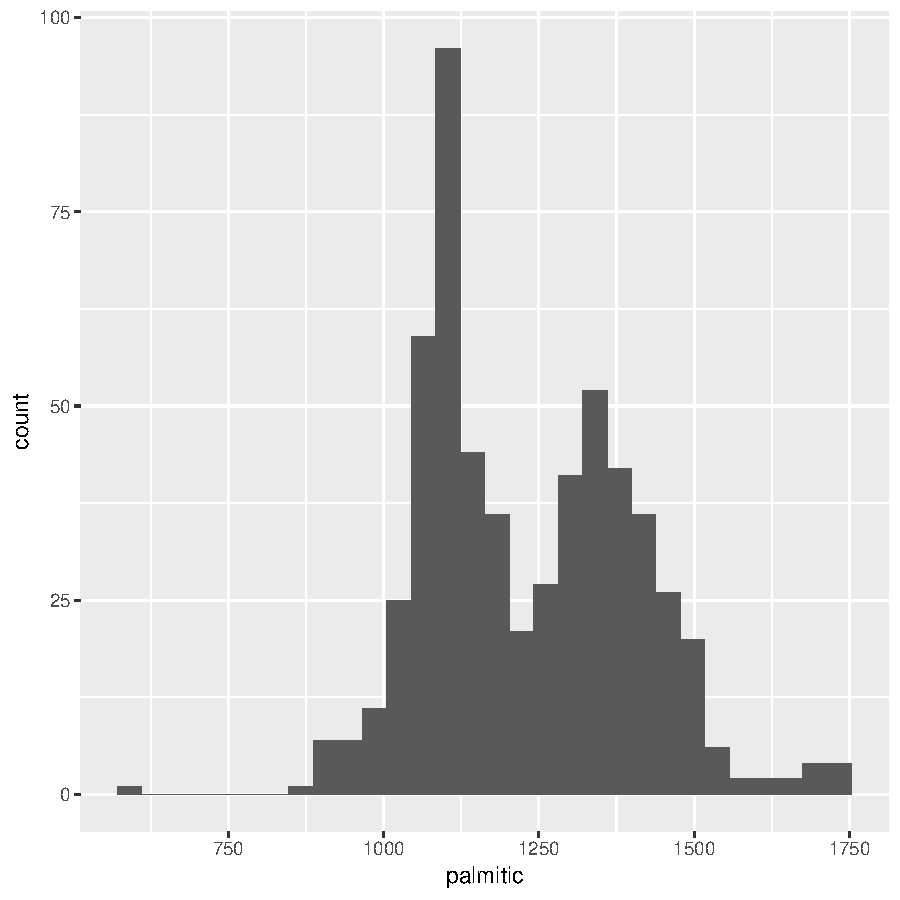
\includegraphics{hw02_bartschi-002}

The histogram appears to be bimodal with a possible outlier below 750.  This of course is not easily interpretable by people, as the bin sizes are not ideal, and the endpoints are not well labeled.

\item (4 Points) 
Create four histograms via {\it ggplot2},
using Sturges, sqrt(n), Scott, and FD breaks.
How many intervals are there in each of the four histograms?
Consider them as small multiples.  So enforce the same scale 
for the horizontal and vertical axes.
Describe these histograms. What is similar, what is different?
Include your final graphs (arranged in a single figure) and your R code. \\

\begin{Schunk}
\begin{Sinput}
> palmitic1 <- olives[,3]
> n <- length(palmitic1)
> h1 <- ggplot(olives, aes(x = palmitic1)) + 
+   geom_histogram(bins = nclass.Sturges(palmitic1)) + 
+   ggtitle("Sturges Breaks") + 
+   theme(plot.title = element_text(hjust = 0.5))
> h2 <- ggplot(olives, aes(x = palmitic1)) + 
+   geom_histogram(bins = as.integer(sqrt(n))) + 
+   ggtitle("Sqrt(n) breaks") + 
+   theme(plot.title = element_text(hjust = 0.5))
> h3 <- ggplot(olives, aes(x = palmitic1)) + 
+   geom_histogram(bins = nclass.scott(palmitic1)) + 
+   ggtitle("Scott breaks") + 
+   theme(plot.title = element_text(hjust = 0.5))
> h4 <- ggplot(olives, aes(x = palmitic1)) + 
+   geom_histogram(bins = nclass.FD(palmitic1)) + 
+   ggtitle("FD breaks") + 
+   theme(plot.title = element_text(hjust = 0.5))
> grid.arrange(h1, h2, h3, h4, nrow = 2)
\end{Sinput}
\end{Schunk}
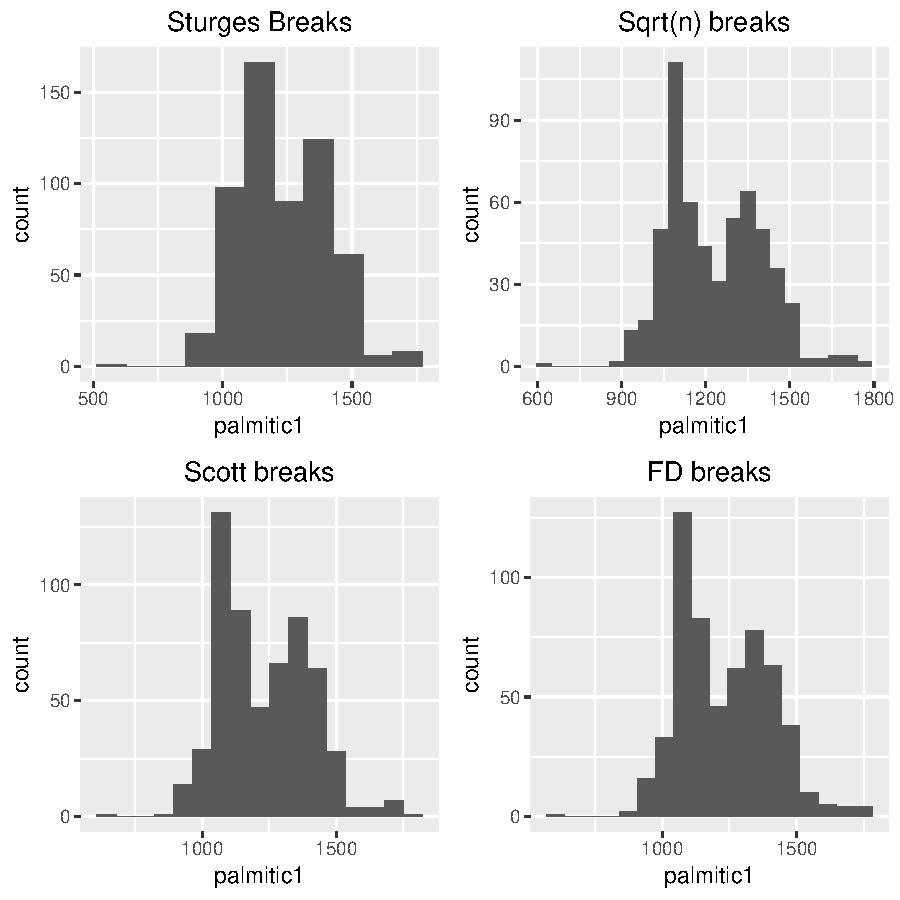
\includegraphics{hw02_bartschi-003}


\item (3 Points) 
Choose one of your four histograms and optimize
it for a human reader via {\it ggplot2}. Make sure to select meaningful 
starting values for the intervals and meaningful interval widths. 
610 (as starting value) and 33.5 (as interval width) are not meaningful
for a human reader. You may end up
with a slightly different number of intervals than what you started with.
Indicate which numbers you selected for the starting value, the number of intervals, and
the interval widths. Further optimize this histogram.
Include your final graph and your R code. 

\begin{Schunk}
\begin{Sinput}
> ggplot(olives, aes(x = palmitic1)) + 
+   geom_histogram(bins = as.integer(sqrt(n)), center = 1000, 
+                  color = 'black', fill = 'white', 
+                  closed = 'left') +
+   xlim(550,1750) + xlab('Palmitic Fat') + 
+   ggtitle("Sqrt(n) breaks") + 
+   theme(plot.title = element_text(hjust = 0.5))
\end{Sinput}
\end{Schunk}
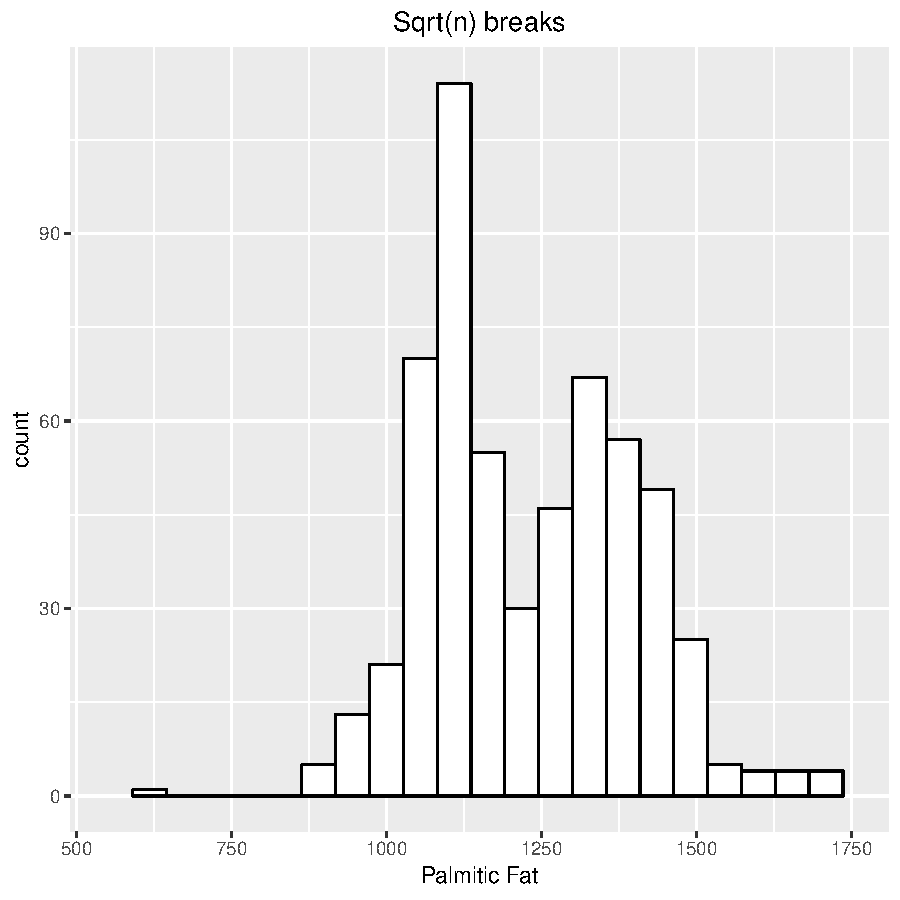
\includegraphics{hw02_bartschi-004}

~\\
\item (3 Points) 
What does baseR do? Work with the same method you used
for your manually optimized histogram in {\it ggplot2}, i.e.,
Sturges, sqrt(n), Scott, or FD breaks. How does the resulting baseR
histogram compare to your optimized one from {\it ggplot2}
with respect to starting value, the number of intervals, and interval widths?
Include your final figure and your R code. 

\begin{Schunk}
\begin{Sinput}
> attach(mtcars)
> par(mfrow=c(2,2))
> hist(olives$palmitic, freq = FALSE, main = "Default
+      (Sturges) Breaks")
> hist(olives$palmitic, breaks = as.integer(sqrt(n)), freq =
+      FALSE, main = "sqrt(n) Breaks")
> hist(olives$palmitic, breaks = "scott", freq = FALSE,
+      main = "Scott Breaks")
> hist(olives$palmitic, breaks = "fd", freq = FALSE,
+      main = "FD Breaks")
\end{Sinput}
\end{Schunk}
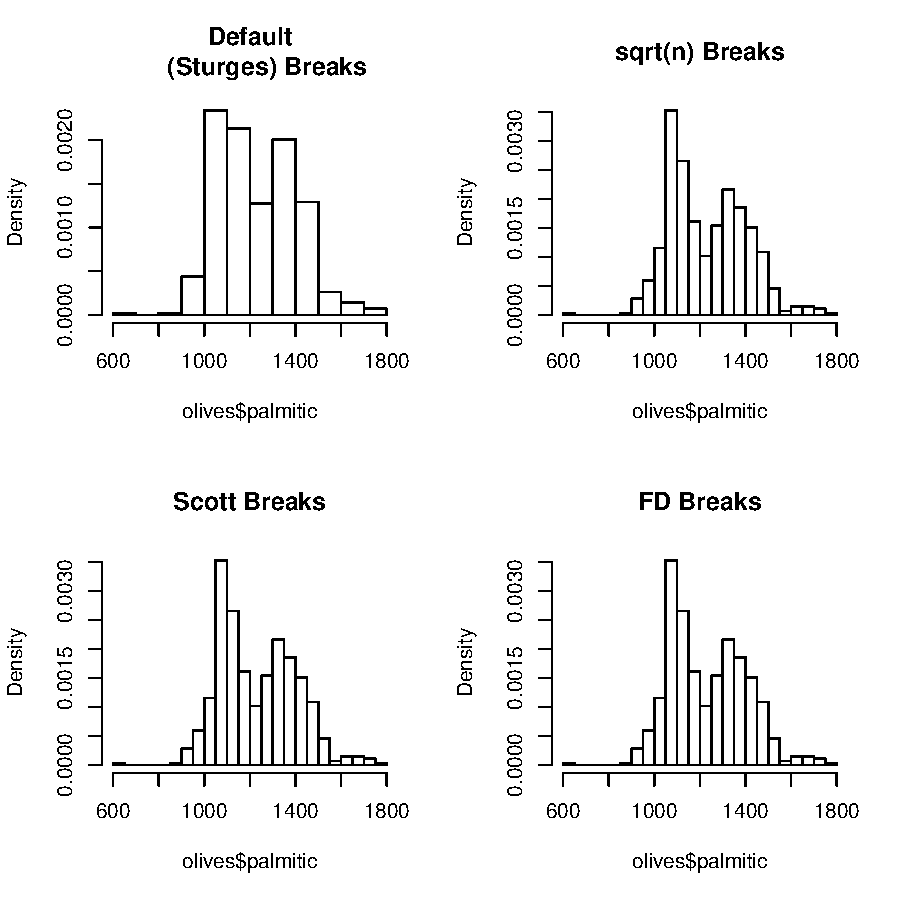
\includegraphics{hw02_bartschi-005}


\item (6 Points) 
Continue with your manually optimized histogram in {\it ggplot2}.
Make sure to switch your histogram to a density scale.
Then create six different plots that overlay six different density curves,
using the default, nrd, ucv, bcv, SJ-ste, and SJ-dpi bandwidths.
Do not further modify the multiplicative bandwidth adjustment (just keep
the default for this). Add a jittered rug plot underneath.
Jitter once and then use the same jittering for all other rug plots as well.
Indicate the amount you use for jittering and why you choose that amount.
Be careful: Your histograms and density curves must make use of the original
data and not of the jittered data.
Include your final graphs (arranged in a single figure) and your R code. 
Describe which of the six bandwiths seems to be the best option to
create a density curve for this variable (use the histogram and rug plot 
for comparison). \\

\begin{Schunk}
\begin{Sinput}
> j1 <- ggplot(olives, aes(x=palmitic1)) +
+     geom_histogram(aes(y = ..density..),
+     bins = nclass.scott(palmitic1),
+     breaks = seq(600, 1700, by = 25), 
+     color = "black",
+     fill="grey",
+     closed = "left") +
+   xlab("Palmitic") + ylab("Count") +
+   geom_density(col = "red") +
+   geom_rug() +
+   ggtitle("Histogram of Palmitic") + 
+   theme(plot.title = element_text(hjust = 0.5))
> j2 <- ggplot(olives, aes(x=palmitic1)) +
+     geom_histogram(aes(y = ..density..),
+     bins = nclass.scott(palmitic1),
+     breaks = seq(600, 1700, by = 25), 
+     color = "black",
+     fill="grey",
+     closed = "left") +
+   xlab("Palmitic") + ylab("Count") +
+   geom_density(bw = "nrd", col = "red") +
+   geom_rug() +
+   ggtitle("Histogram of Palmitic") + 
+   theme(plot.title = element_text(hjust = 0.5))
> j3 <- ggplot(olives, aes(x=palmitic1)) +
+     geom_histogram(aes(y = ..density..),
+     bins = nclass.scott(palmitic1),
+     breaks = seq(600, 1700, by = 25), 
+     color = "black",
+     fill="grey",
+     closed = "left") +
+   xlab("Palmitic") + ylab("Count") +
+   geom_density(bw = "ucv", col = "red") +
+   geom_rug() +
+   ggtitle("Histogram of Palmitic") + 
+   theme(plot.title = element_text(hjust = 0.5))
> j4 <- ggplot(olives, aes(x=palmitic1)) +
+     geom_histogram(aes(y = ..density..),
+     bins = nclass.scott(palmitic1),
+     breaks = seq(600, 1700, by = 25), 
+     color = "black",
+     fill="grey",
+     closed = "left") +
+   xlab("Palmitic") + ylab("Count") +
+   geom_density(bw = "bcv", col = "red") +
+   geom_rug() +
+   ggtitle("Histogram of Palmitic") + 
+   theme(plot.title = element_text(hjust = 0.5))
> j5 <- ggplot(olives, aes(x=palmitic1)) +
+     geom_histogram(aes(y = ..density..),
+     bins = nclass.scott(palmitic1),
+     breaks = seq(600, 1700, by = 25), 
+     color = "black",
+     fill="grey",
+     closed = "left") +
+   xlab("Palmitic") + ylab("Count") +
+   geom_density(bw = "SJ-ste", col = "red") +
+   geom_rug() +
+   ggtitle("Histogram of Palmitic") + 
+   theme(plot.title = element_text(hjust = 0.5))
> j6 <- ggplot(olives, aes(x=palmitic1)) +
+     geom_histogram(aes(y = ..density..),
+     bins = nclass.scott(palmitic1),
+     breaks = seq(600, 1700, by = 25), 
+     color = "black",
+     fill="grey",
+     closed = "left") +
+   xlab("Palmitic") + ylab("Count") +
+   geom_density(bw = "SJ-dpi", col = "red") +
+   geom_rug() +
+   ggtitle("Histogram of Palmitic") + 
+   theme(plot.title = element_text(hjust = 0.5))
> grid.arrange(j1, j2, j3, j4, j5, j6, nrow = 3)
\end{Sinput}
\end{Schunk}
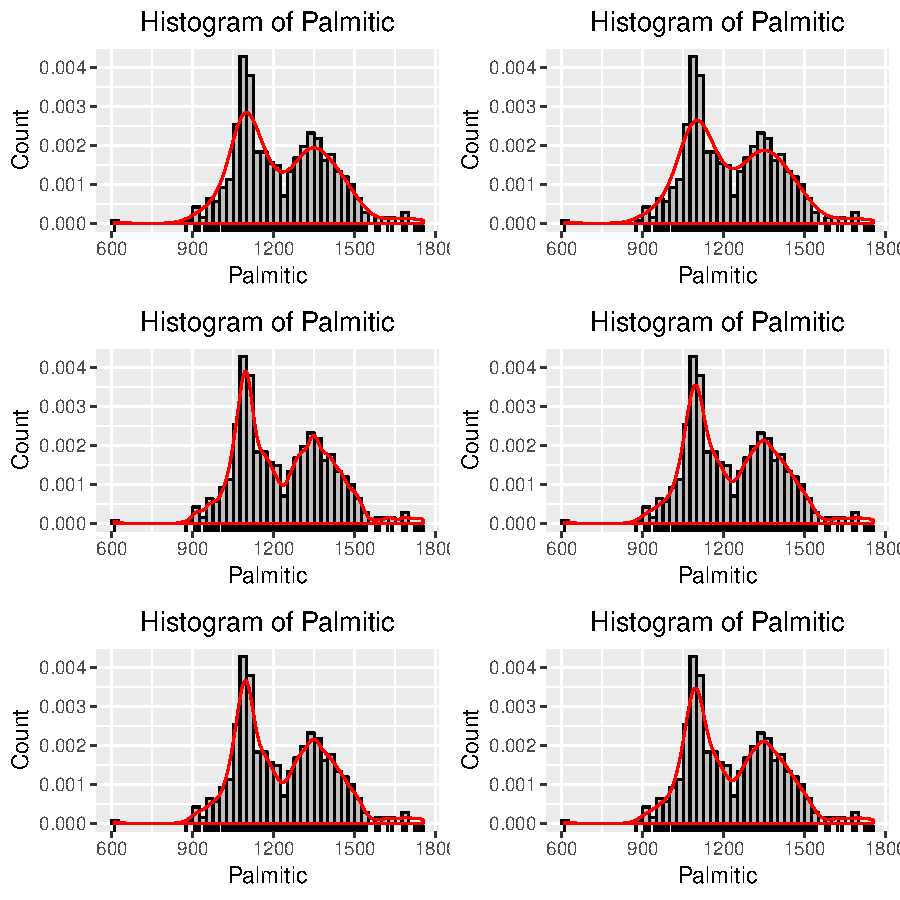
\includegraphics{hw02_bartschi-006}

\item (6 Points)
Now focus on the three different regions: Create three graphs side-by-side
that show 
(a) boxplots for the three regions; 
(b) violin plots for the three regions; and
(c) letter-valued boxplots for the three regions.
Make sure that the regions are ordered as North (left), Sardinia (center), and South (right)
in your three graphs. 
All individual graphs should extend in vertical (top-bottom) direction.
Thus, use the same scale for the vertical axis.
Ensure that the graphs follow the small multiples principle.
So, when you use a specific color for a region, you have to use the same color
in all other graphs for that region. 
Include your final graphs (arranged side-by-side) and your R code.
What can we learn about similarities and differences of the distributions
in the three different regions from these graphs?

\begin{Schunk}
\begin{Sinput}
> p1 <- ggplot(olives, aes(x = Region, y = palmitic, fill = 
+                            Region))  + geom_boxplot() +
+   theme(axis.title.y = element_blank(), legend.position = 
+           "none", plot.title = element_text(hjust = 0.5)) + 
+   ggtitle("Palmitic (box)")
> p2 <- ggplot(olives, aes(x = Region, y = palmitic, fill = 
+                            Region))  + 
+   theme(axis.title.y = element_blank(), axis.text.y = 
+           element_blank(),axis.ticks.y = element_blank(), 
+         legend.position = "none") +
+   geom_violin() + ggtitle("Palmitic (violin)") + 
+   theme(plot.title = element_text(hjust = 0.5))
> p3 <- ggplot(olives, aes(x = Region, y = palmitic, fill = 
+                            Region))  + geom_lv() +
+   theme(axis.title.y = element_blank(), axis.text.y = 
+           element_blank(),axis.ticks.y = element_blank(),
+         legend.position = "none") + ggtitle("Palmitic (letter)") + 
+   theme(plot.title = element_text(hjust = 0.5))
> grid.arrange(p1, p2, p3, nrow = 1)
\end{Sinput}
\end{Schunk}
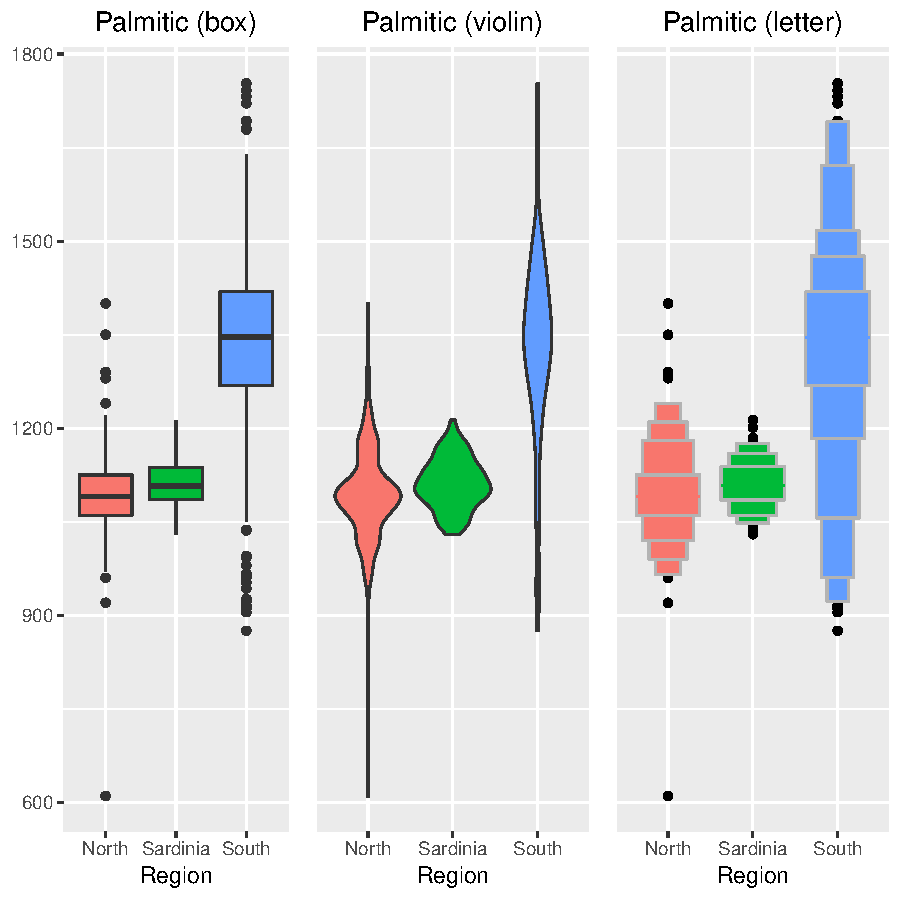
\includegraphics{hw02_bartschi-007}


\newpage


\item (3 Points)
Are the distributions in the three different regions approximately Normal?
Construct Q-Q plots and answer this question.
Include your final graphs (arranged in a meaningful way) and your R code.
%par(mfrow = c(3,1))
%qqnorm(olives$palmitic[c(1:246,437:513)],title = 'meh')
%qqnorm(olives$palmitic[c(247:320,514:537)])
%qqnorm(olives$palmitic[c(321:436,538:572)])

\begin{Schunk}
\begin{Sinput}
> ggplot(olives, aes(sample = palmitic, colour = Region)) + 
+   stat_qq() +
+   ggtitle("Q-Q Plots by Region") +
+   theme(plot.title = element_text(hjust = 0.5))
\end{Sinput}
\end{Schunk}
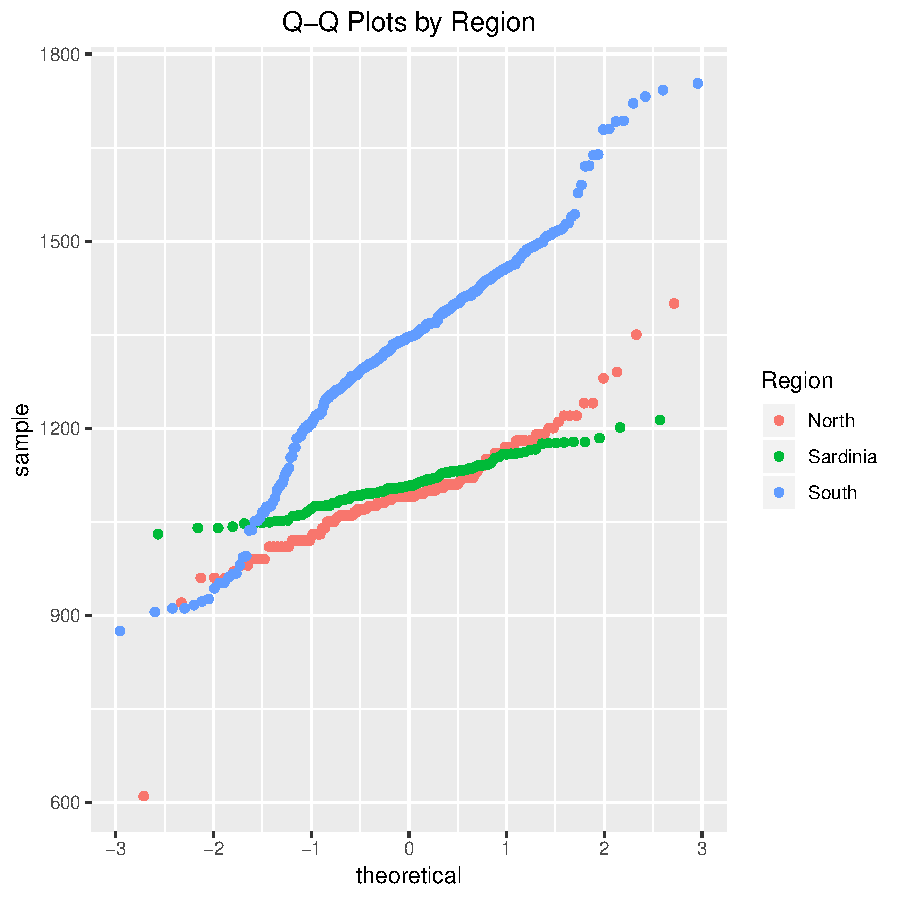
\includegraphics{hw02_bartschi-008}


\item (3 Points)
Construct three empirical cdfs (ecdfs) for the three different regions 
and overlay them in the same graph. If you used colors before,
use the same colors again for the three regions. In any case, include
a meaningful legend. How similar (or different) are those ecdfs?
Include your final graph and your R code.

\begin{Schunk}
\begin{Sinput}
> ggplot(olives, aes(x = palmitic, colour = Region)) +
+   stat_ecdf() +
+   ggtitle("ECDF Plot") +
+   theme(plot.title = element_text(hjust = 0.5))
\end{Sinput}
\end{Schunk}
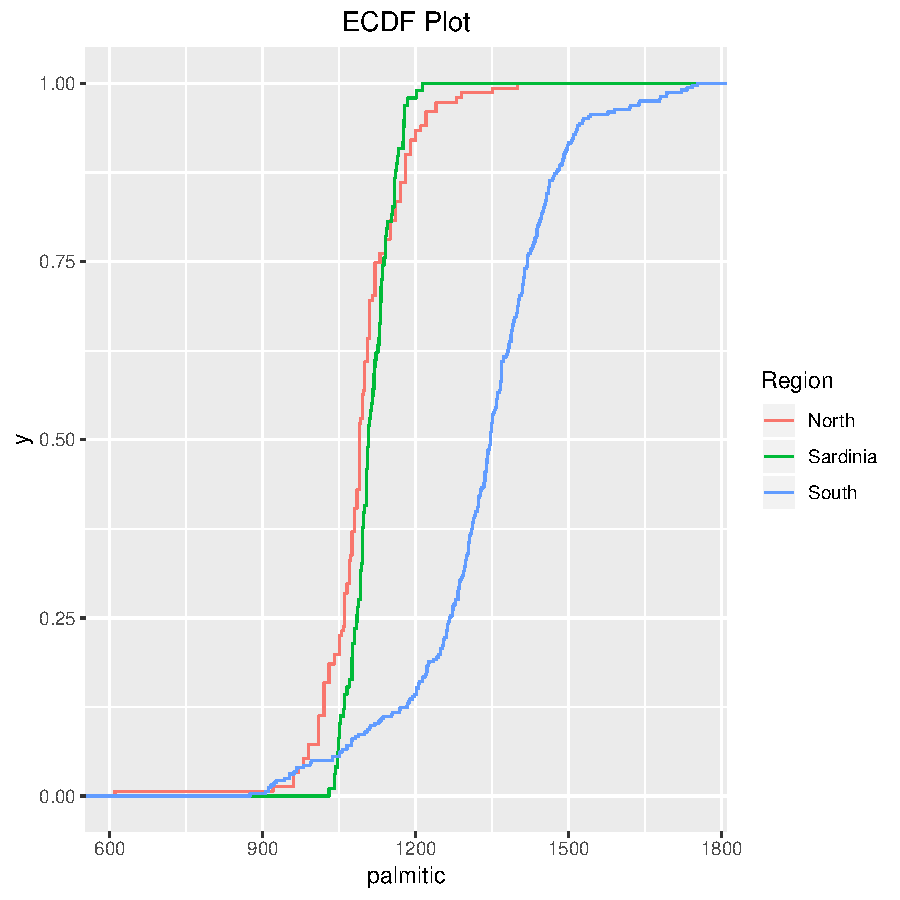
\includegraphics{hw02_bartschi-009}


\item (6 Points)
Summarize your results. What did we learn about  the distribution of the
palmitic fat overall? And what can we say about the regions? Which 
are similar, which are different (if any). If necessary, repeat some
of your previous results and observations here. Your summary should be about
1/2 to 3/4 of a page long.

\break

\underline{Answer:}

From the variety of graphics we produced, we were able to learn the following:

The distribution of the palmitic fatty acids across the three regions combined appears to have a bimodal distribution.  We observed this when we did our first histograms.

The distribution of the palmitic acids in the North appears to be roughly linear, with the possibility of some outliers.  This is infered from both the box and letter box plots, and from the QQ-Plot.

the distribution of the palmitic acids in the Sardinia Region appears to be strongly normal from our Q-Q plot, and furthermore, Sardinia and the Southern region appear to be similar in distribution when considering nearly all of our plots.

On the other hand, the Southern region appears to be highly non-normal, and distributed significantly differently that the other two regions.  Furthermore, considering that the number of observations from the Southern region is double the number from the North and more than triple the number of observations from Sardinia, this region alone contributed highly to the second mode in our overall graph.  Removing this region from consideration would likely yield an approximately normal histogram

\end{enumerate}



\newpage


\item (16 Points) {\bf Hair and Eye Colors:}
In this question, you have to work with the {\it HairEyeColor} data set (from  baseR).
It shows the distribution of hair color, eye color, and sex in 592 statistics students.
See the {\it HairEyeColor} help page and 
any of the cited references
for further details.

\begin{enumerate}
\item (6 Point) Create six different mosaic plots that show all possible
layouts for the three variables, using baseR. Also show the standardized residuals,
based on the assumption that all three variables are independent.
Include your figures and your R code. \\

\underline{Answer:}
{\scriptsize
\begin{Schunk}
\begin{Sinput}
> data("HairEyeColor")
> mosaicplot(HairEyeColor, shade = TRUE)
\end{Sinput}
\end{Schunk}
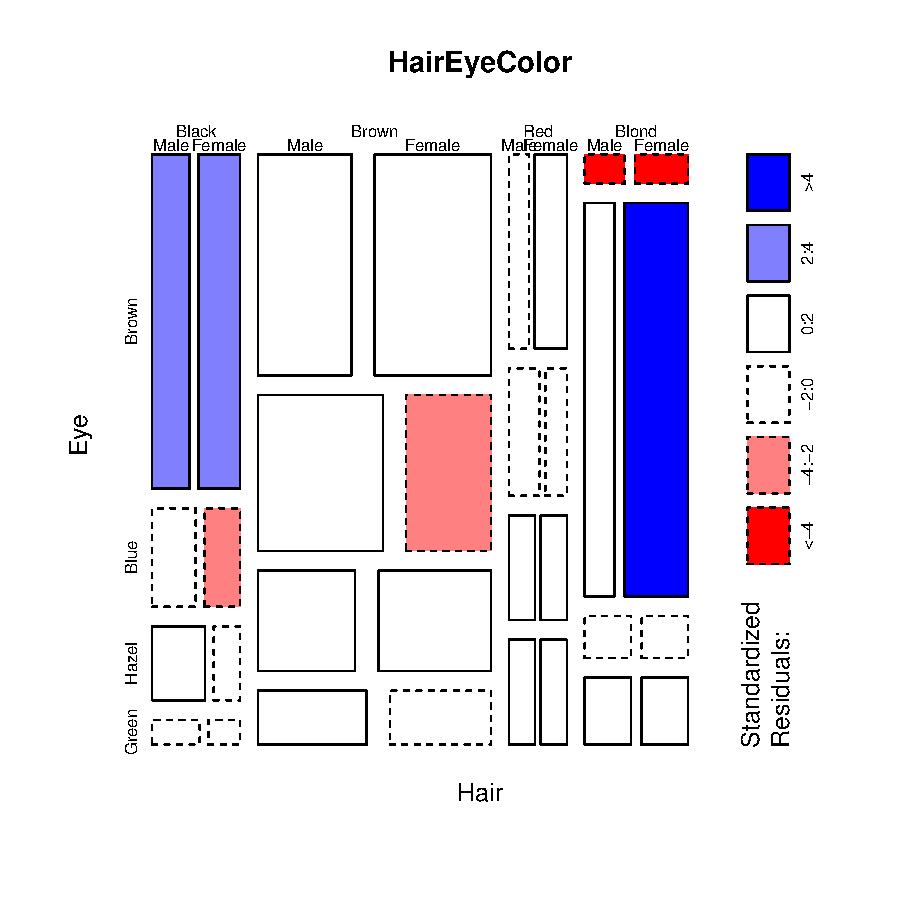
\includegraphics{hw02_bartschi-010}
\newpage
\begin{Schunk}
\begin{Sinput}
> mosaicplot(aperm(HairEyeColor,3:1), shade = TRUE)
\end{Sinput}
\end{Schunk}
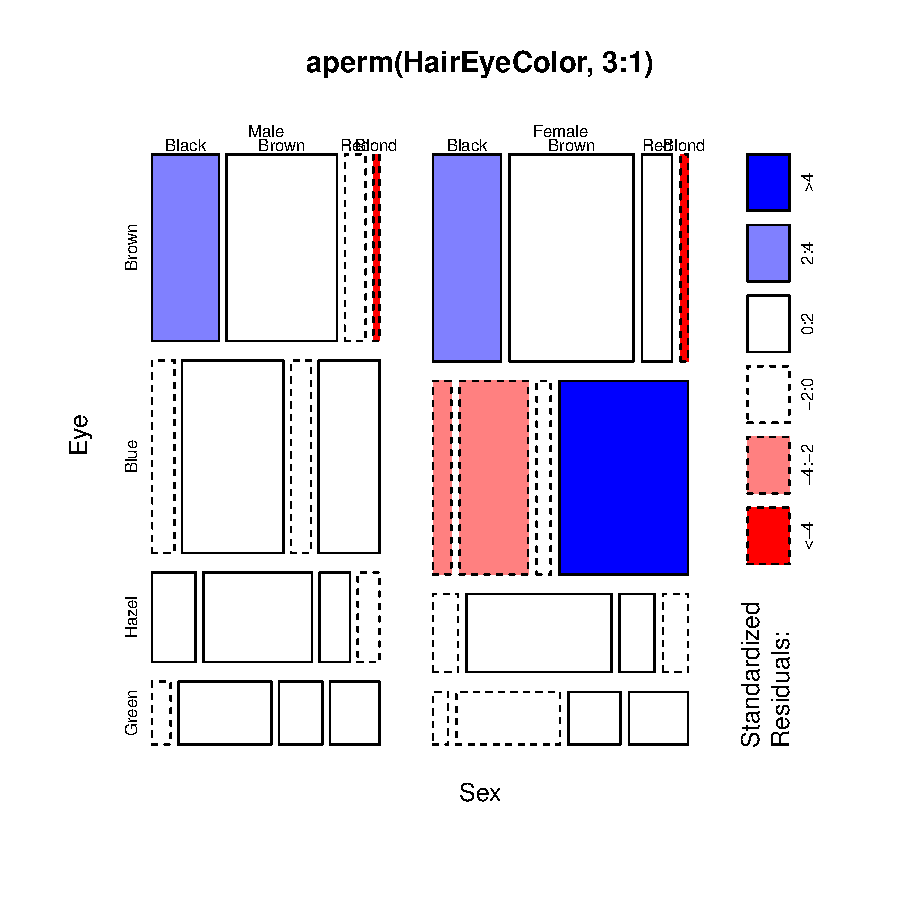
\includegraphics{hw02_bartschi-011}
\newpage
\begin{Schunk}
\begin{Sinput}
> mosaicplot(aperm(HairEyeColor,c(2,3,1)), shade = TRUE)
\end{Sinput}
\end{Schunk}
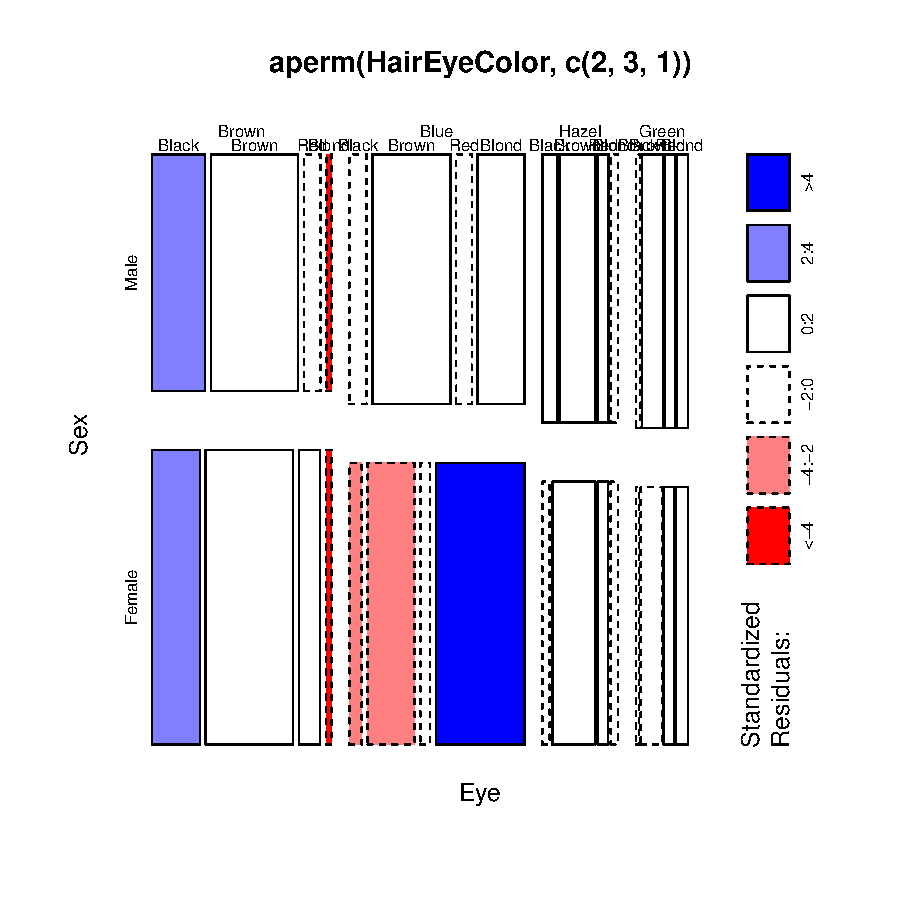
\includegraphics{hw02_bartschi-012}
\newpage
\begin{Schunk}
\begin{Sinput}
> mosaicplot(aperm(HairEyeColor,c(2,1,3)), shade = TRUE)
\end{Sinput}
\end{Schunk}
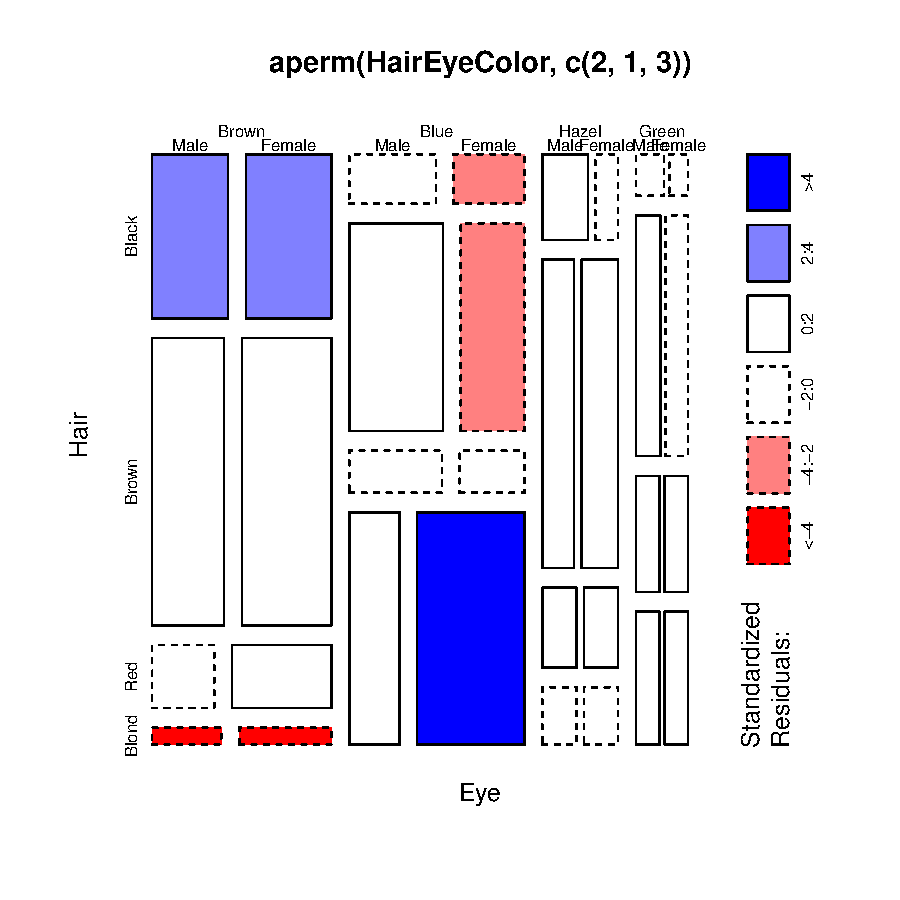
\includegraphics{hw02_bartschi-013}
\newpage
\begin{Schunk}
\begin{Sinput}
> mosaicplot(aperm(HairEyeColor,c(1,2,3)), shade = TRUE)
\end{Sinput}
\end{Schunk}
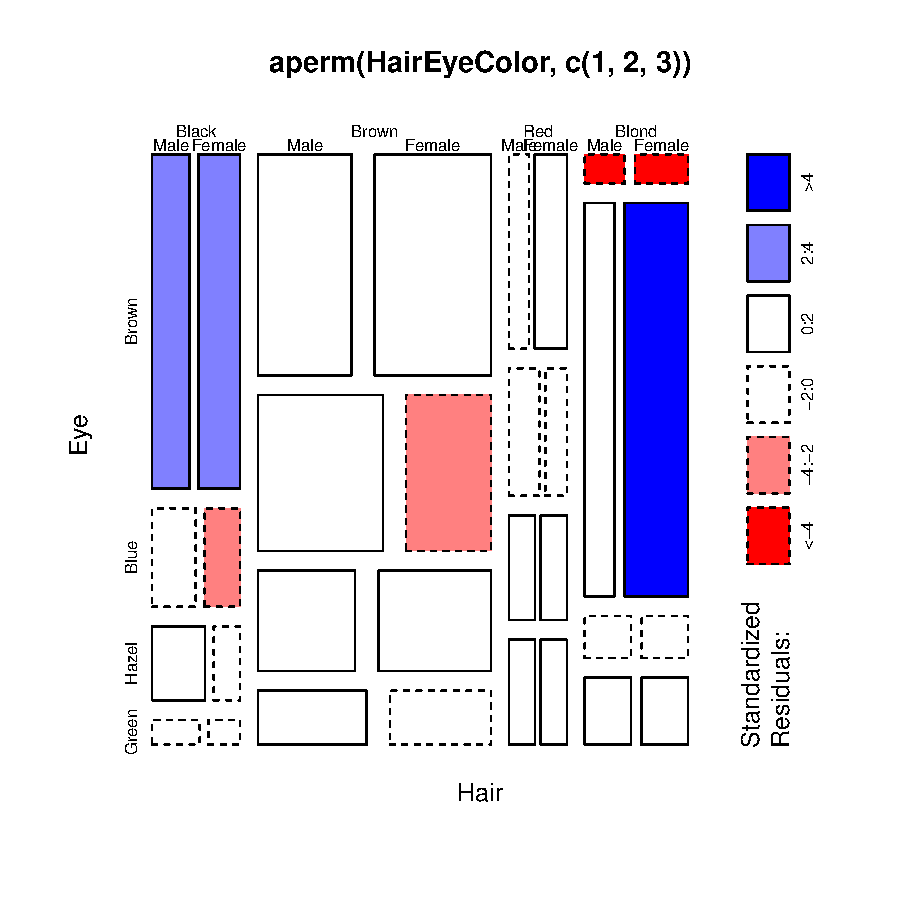
\includegraphics{hw02_bartschi-014}
\newpage
\begin{Schunk}
\begin{Sinput}
> mosaicplot(aperm(HairEyeColor,c(3,2,1)), shade = TRUE)
\end{Sinput}
\end{Schunk}
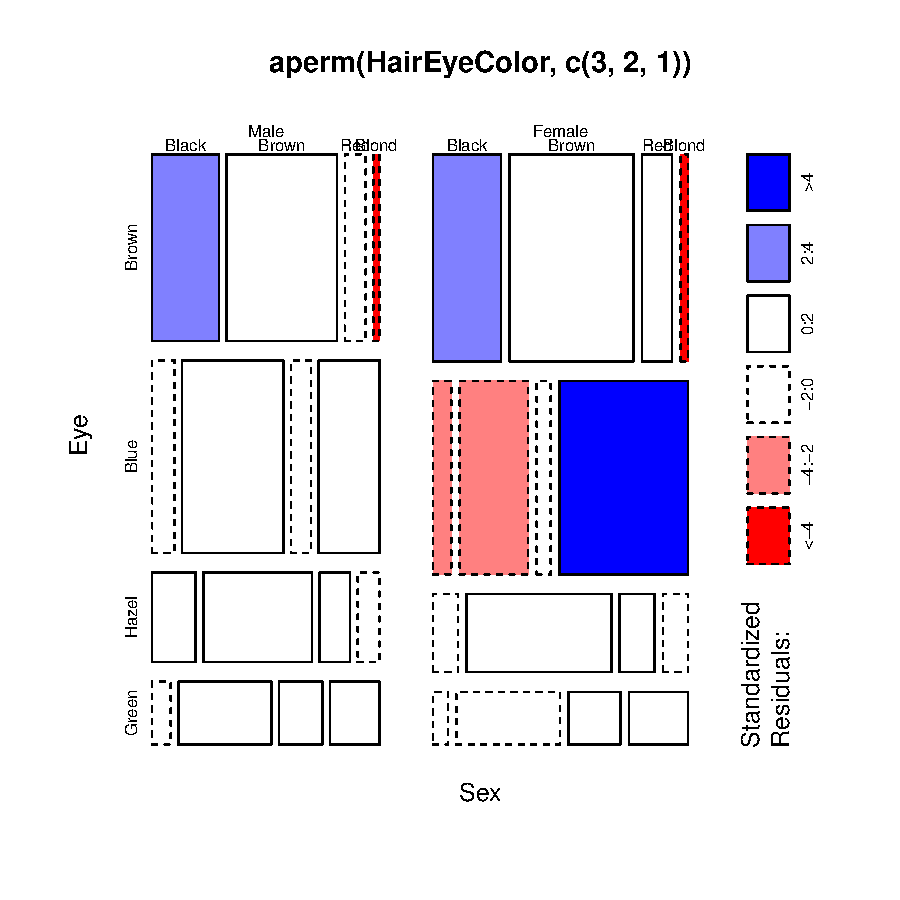
\includegraphics{hw02_bartschi-015}
}


\item (5 Point) Overall, each of your mosaic plots above should show seven colored areas.
These may relate to hair color, eye color, or sex. Six of the seven shaded areas 
come in pairs (i.e., three pairs of two related areas each) 
and one is a unique combination of the three variables.
Optimize (i.e., add labels, etc.) the mosaic plot that best displays the pairs and 
the unique combination. 
Pairs should be located next to each other and not in different regions of the plot.
There are two (of the six) mosaic plots that meet this condition and could be optimized.
You only have to optimize one.
Include your resulting figure and your R code. \\

\begin{Schunk}
\begin{Sinput}
> mosaicplot(aperm(HairEyeColor,c(2,1,3)), shade = TRUE, main = 'Hair and Eye Color by Gender', xlab = 'Eye Color', ylab = 'Hair Color')
\end{Sinput}
\end{Schunk}
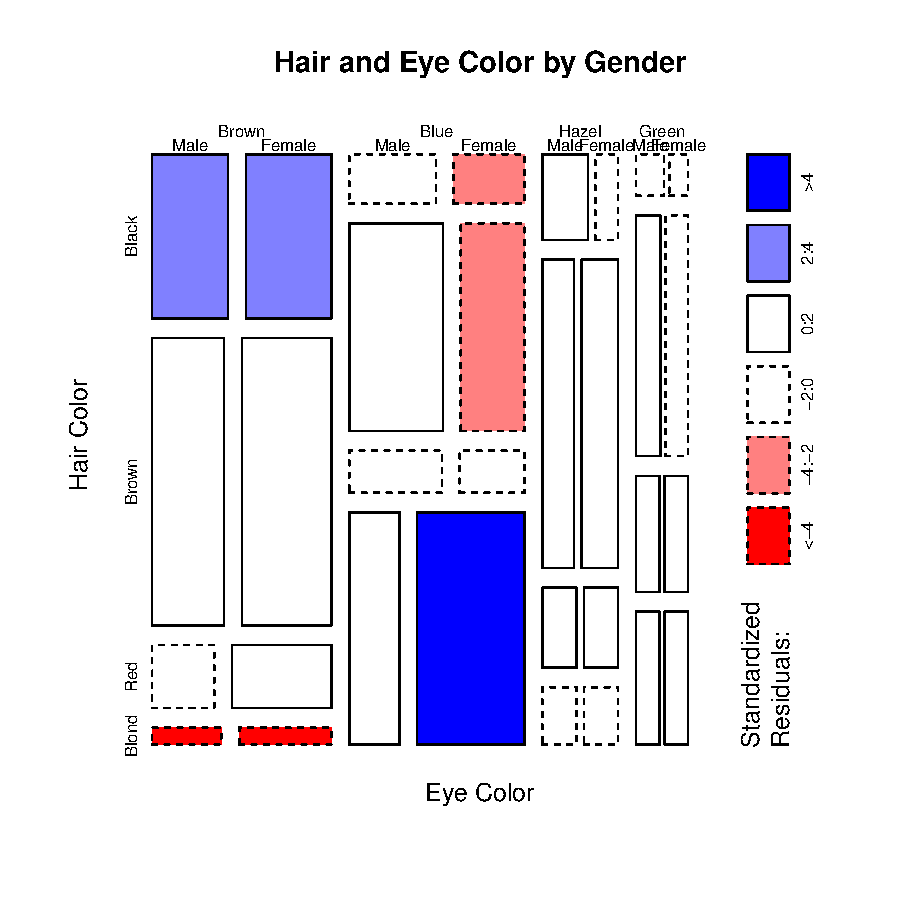
\includegraphics{hw02_bartschi-016}


\item (5 Point) Describe and explain your mosaic plot from (b) above. 
What can be seen? Assume that a reader is not familiar with mosaic plots,
so you have to start with the basic layout you used. How can we best interpret
the three pairs and the unique combination? Isn't there an important lurking variable that
is missing from this data set, but that would help to even better explain the
observed pattern? Which variable is this --- and how could it be used to explain
the pattern?

\end{enumerate}


\newpage


\item (10 Points) {\bf Barley Data:}
Reconstruct and optimize the final version of the {\it barley} data dot plot
from Section 5.7 (Dot Charts for Univariate Data) in our lecture notes, using {\it ggplot2}. 
Make sure that you use the same sorting (of the varieties and of the sites) and colors (for the years)
as in our version of this plot
that was created via the {\it lattice} dotplot function.
Include your final figure and your R code. \\


\underline{Answer:}
{\scriptsize
\begin{Schunk}
\begin{Sinput}
> data(barley)
> ggplot(barley, aes(x = yield , y = variety, fill = year)) +
+   geom_dotplot(binaxis = 'y') +
+   facet_grid(barley$site) 
\end{Sinput}
\end{Schunk}
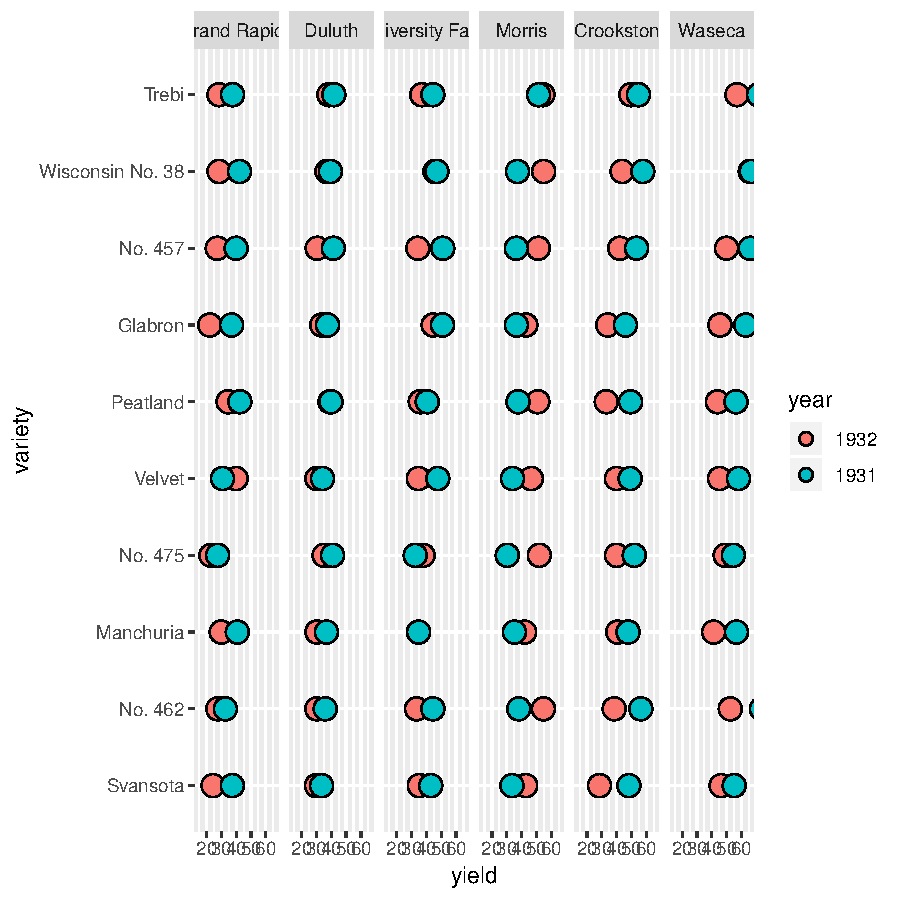
\includegraphics{hw02_bartschi-017}
}


\end{enumerate}


\newpage


\noindent{\Large \bf General Instructions}~\\


\begin{enumerate}
\item Create a single html or pdf document, using R Markdown, Sweave, or knitr.
You only have to submit this one document.

\item Include a title page that contains your name, your A-number, the number of
the assignment, the submission date, and any other relevant information.

\item Start your answers to each main question on a new page (continuing with the next
part of a question on the same page is fine). 
Clearly label each question and question part.

\item Before you submit your homework, check that you
follow all recommendations from Google's R Style Guide
(see \url{https://google.github.io/styleguide/Rguide.xml}). 
Moreover, make sure that your R code is consistent, i.e., that you use the same
type of assignments and the same type of quotes throughout your entire homework.

\item Give credit to external sources, such as stackoverflow or help pages. Be specific
and include the full URL where you found the help (or from which help page you got 
the information). Consider R code from such sources as ``legacy code or third-party code'' 
that does not have to be adjusted to Google's R Style (even though it would be nice,
in particular if you only used a brief code segment).

\item {\bf Not following the general instructions outlined above will result in point deductions!}

\item For general questions related to this homework, please
use the corresponding discussion board in Canvas! I will try to
reply as quickly as possible. Moreover, if one of you knows
an answer, please post it. It is fine to refer to web pages
and R commands, but do not provide the exact R command with all required arguments
or which of the suggestions from a stackoverflow web page eventually worked for you! 
This will be the task for each individual student!

\item Submit your single html or pdf file via Canvas by the submission deadline.
Late submissions will result in point deductions as outlined on the syllabus.

\end{enumerate}


\end{document}

